\subsection{Измерение времени выполнения параллельных программ}
\label{subsec:execution-time-measurement}

\textbf{Инструменты измерения времени.} Измерение времени работы программы в языке С не является сложной проблемой, однако при параллельном программировании возникает ряд специфических сложностей при выполнении этой операции. Далеко не все функции, пригодные для измерения времени работы последовательной программы, подойдут для измерения времени работы многопоточной программы. 

Например, если в однопоточной программе для измерения времени работы участка кода использовать функции ctime или localtime, то они успешно справятся с поставленной задачей. Однако после распараллеливания этого участка кода возможно возникновение трудно идентифицируемых проблем с неправильным измерением времени, т.к. обе указанные функции имеют внутреннюю static-переменную, которая при попытке изменить её одновременно несколькими потоками может принять непредсказуемое значение.

С целью решить описанную проблему в некоторых C-компиляторах (например, gcc) были реализованы потокобезопасные (thread-safe, reen\-trant) версии этих функций: ctime\_r и localtime\_r. К сожалению, эти функции доступны не во всех компиляторах. Например, в компиляторе Visual Studio аналогичную проблему решили использованием функций с совсем иными именами и API: Get\-Tick\-Count, Get\-Local\-Time, Get\-System\-Time. Перечислим для полноты изложения некоторые другие gcc-функции, которые также позволяют измерять время: time, get\-r\-usage, gm\-time, get\-time\-of\-day.

Ещё одна стандартная С-функция clock также не может быть использована для измерения времени выполнения многопоточных программ. Однако причина этого не в отсутствии реентерабельности, а в особенностях способа, которым эта функция рассчитывает прошедшее время: clock возвращает число тиков процессора, которые были выполнены при работе программы суммарно всеми её потоками. Очевидно, что это число остается почти неизменным при выполнении программы разным числом потоков (<<почти>>, т.к. накладные расходы на создание, удаление и управление потоками предлагается в целях упрощения изложения считать несущественными).

В итоге оказалось, что удовлетворительного \textit{кросс-платформенного} решения для потокобезопасного измерения времени с высокой точностью (до микросекунд) средствами чистого языка С пока не существует. Проблему, однако, можно решить, используя сторонние библиотеки, выбирая те из них, которые имеют реализацию на целевых платформах.

Выгодно выделяется среди таких библиотек система OpenMP, которая реализована в абсолютном большинстве современных компиляторов для всех современных операционных систем. В OpenMP есть две функции для измерения времени: omp\_get\_wtime и omp\_get\_wtick, которые можно использовать в С-программах, если подключить заголовочный файл omp.h и при компиляции указать нужный ключ (например, в gcc это ключ <<-fopenmp>>).

\textbf{Погрешность измерения времени.} Другим интересным моментом при измерении времени работы параллельной программы является способ, с помощью которого исследователь исключает из замеров различные случайные погрешности, неизбежно возникающие при эксперименте в работающей операционной системе, которая может начать процесс обновления или оптимизации, не уведомляя пользователя. Общепринятыми является способ, при котором исследователь проводит не один, а сразу N экспериментов с параллельной программой, не меняя исходные данные. Получается N замеров времени, которые в общем случае будут различными вследствие различных случайных факторов, влияющих на проводимый эксперимент. Далее чаще всего используется один из следующих методов:

\begin{enumerate}
    \item\textit{Расчёт доверительного интервала:} с учётом всех N измерений рассчитывается доверительный интервал, например, с помощью метода Стьюдента.
    \item\textit{Поиск минимального замера:} среди N измерений выбирается наименьшее и именно оно используется в качестве окончательного результата.
\end{enumerate}

Первый метод даёт корректный результат, только если ошибки замеров распределены по нормальному закону. Чаще всего это так, поэтому применение метода оправдано и также позволяет получить дополнительную информацию о возможном применении тестируемой программы в живых условиях работающей ОС.

Второй метод не предъявляет требований к виду закона распределения ошибки измерений и этим выгодно отличается от предыдущего. Кроме того, при больших N выбор минимального замера позволит с большой вероятностью исключить из эксперимента все фоновые влияния операционной системы и получить в качестве результата точное измерение времени работы программы в идеальных условиях. 

\textbf{Практический пример.} Сравним на примере описанные выше методы избавления от погрешности экспериментальных замеров времени. Будем измерять накладные расходы OpenMP на создание и удаление потоков следующим образом:

\inputminted{c++}{listings/OpenMPExampleTimeMeasurement.cpp}

В строке 2 мы даём OpenMP указание, чтобы при входе в параллельную область, расположенную далее в программе, было создано i потоков. Если не давать этого указания, OpenMP создаст число потоков по числу доступных в системе вычислителей (ядер или логических процессоров). В строке 4 мы запускаем параллельную область программы, OpenMP создаёт i потоков. В строке 5 мы даём указание выполнять последующую простейшую инструкцию лишь в одном потоке (остальные потоки не будут делать никакой работы. Это нужно, чтобы в замеряемое время работы попали только расходы на создание/удаление потоков, а все прочие расходы терялись бы на их фоне. В строке 6 заканчивается параллельная область, OpenMP удаляет из памяти i потоков. Более подробное описание использованных команд OpenMP можно найти в разделе~\ref{OpenMP:section} \textit{<<Технология OpenMP>>} данного учебного  пособия.

Эксперименты с приведённой программой проводились на компьютере с процессором Intel Core i5 (4 логических процессора) с 8 гигабайт ОЗУ в операционной системе Debian Wheezy. Опытным путём было выявлено, что использованная операционная система на доступной аппаратной платформе не может создать более 381 потока в OpenMP-программе (этим объясняется значение в строке 1). Было проведено в общей сложности N=100 экспериментов, результаты которых обрабатывались каждым из двух описанных методов. Полученные результаты приведены на рисунке~\ref{fig:openmp-creating-threads-overhead}.

\begin{figure}[H]
    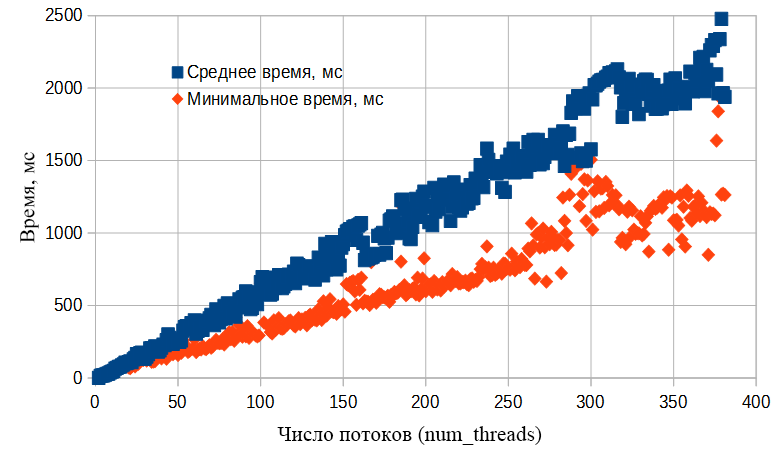
\includegraphics[width=1\linewidth]{OpenMPExpensesOnCreatingThreads}
    \caption{Результаты измерения накладных расходов OpenMP при создании и удалении потоков}
    \label{fig:openmp-creating-threads-overhead}
\end{figure} 

По оси ординат откладывается измеренная величина (T2 - T1) в миллисекундах, по оси абсцисс – значения переменной i, означающие число создаваемых потоков. Верхний график, состоящий из синих квадратов, показывает усреднённую величину (T2 - T1) по 100 проведённым экспериментам. Доверительный интервал при этом не показан, т.к. он загромождал бы график, не добавляя информативности, однако ширина доверительного интервала с уровнем доверия 90\% приблизительно соответствует разбросу по вертикали квадратов верхнего графика для соседних значений i.

Нижний график, состоящий из ромбов, представляет собой минимальные из 100 проведённых замеров величины (T2 -  T1) для указанных на оси абсцисс значений i. Видим, что даже большого числа экспериментов оказалось недостаточно, чтобы нижний график имел бы гладкую непрерывную структуру без заметных флуктуаций.
